%%%%%%%%%%%%%%%%%%%%%%%%%%%  2  %%%%%%%%%%%%%%%%%%%%%%%%%%%
\section{Low-power, high-speed transceivers for network-on-chip
communication \cite{schinkel2009low}} \label{ss:schinkel2009low}
%%%%%%%%%%%%%%%%%%%%%%%%%%%  2  %%%%%%%%%%%%%%%%%%%%%%%%%%%
The interconnect of a chip has become a bottleneck regarding speed, power en reliability of chip due to its high capacitance and high resistance. \acc{noc} technology is a good candidate for future progress.
\ac{noc} is for instance more power efficient and allows for different kinds of synchronous and asynchronous techniques.

% IETS ZEGGEN OVER TOEGEPASTE TECHNOLOGIE
\motive
However, when using \acsp{noc} still a lot of power is consumed.
For instance, the on-chip network consumes $39\%$ of the total chip power is consumed \cite{vangal20075}.
It is proposed that a \ac{noc} can benefit from advanced \textit{link-transceivers}.

\objective
In this paper earlier proposed techniques by the authors (\cite{mensink20070}) to decrease the power consumption and to increase the data-rate are applied to \ac{noc} applications.
Tests show a reduced link power of 3.3 times and an increased the data-rate of 80\%.

\summary
In the process of applying the aforementioned optimization's some simplifying assumptions were made. 
For instance, a wire length of 2mm is assumed everywhere. 
The receiver equalization is omitted.

\begin{figure}	\centering
	
	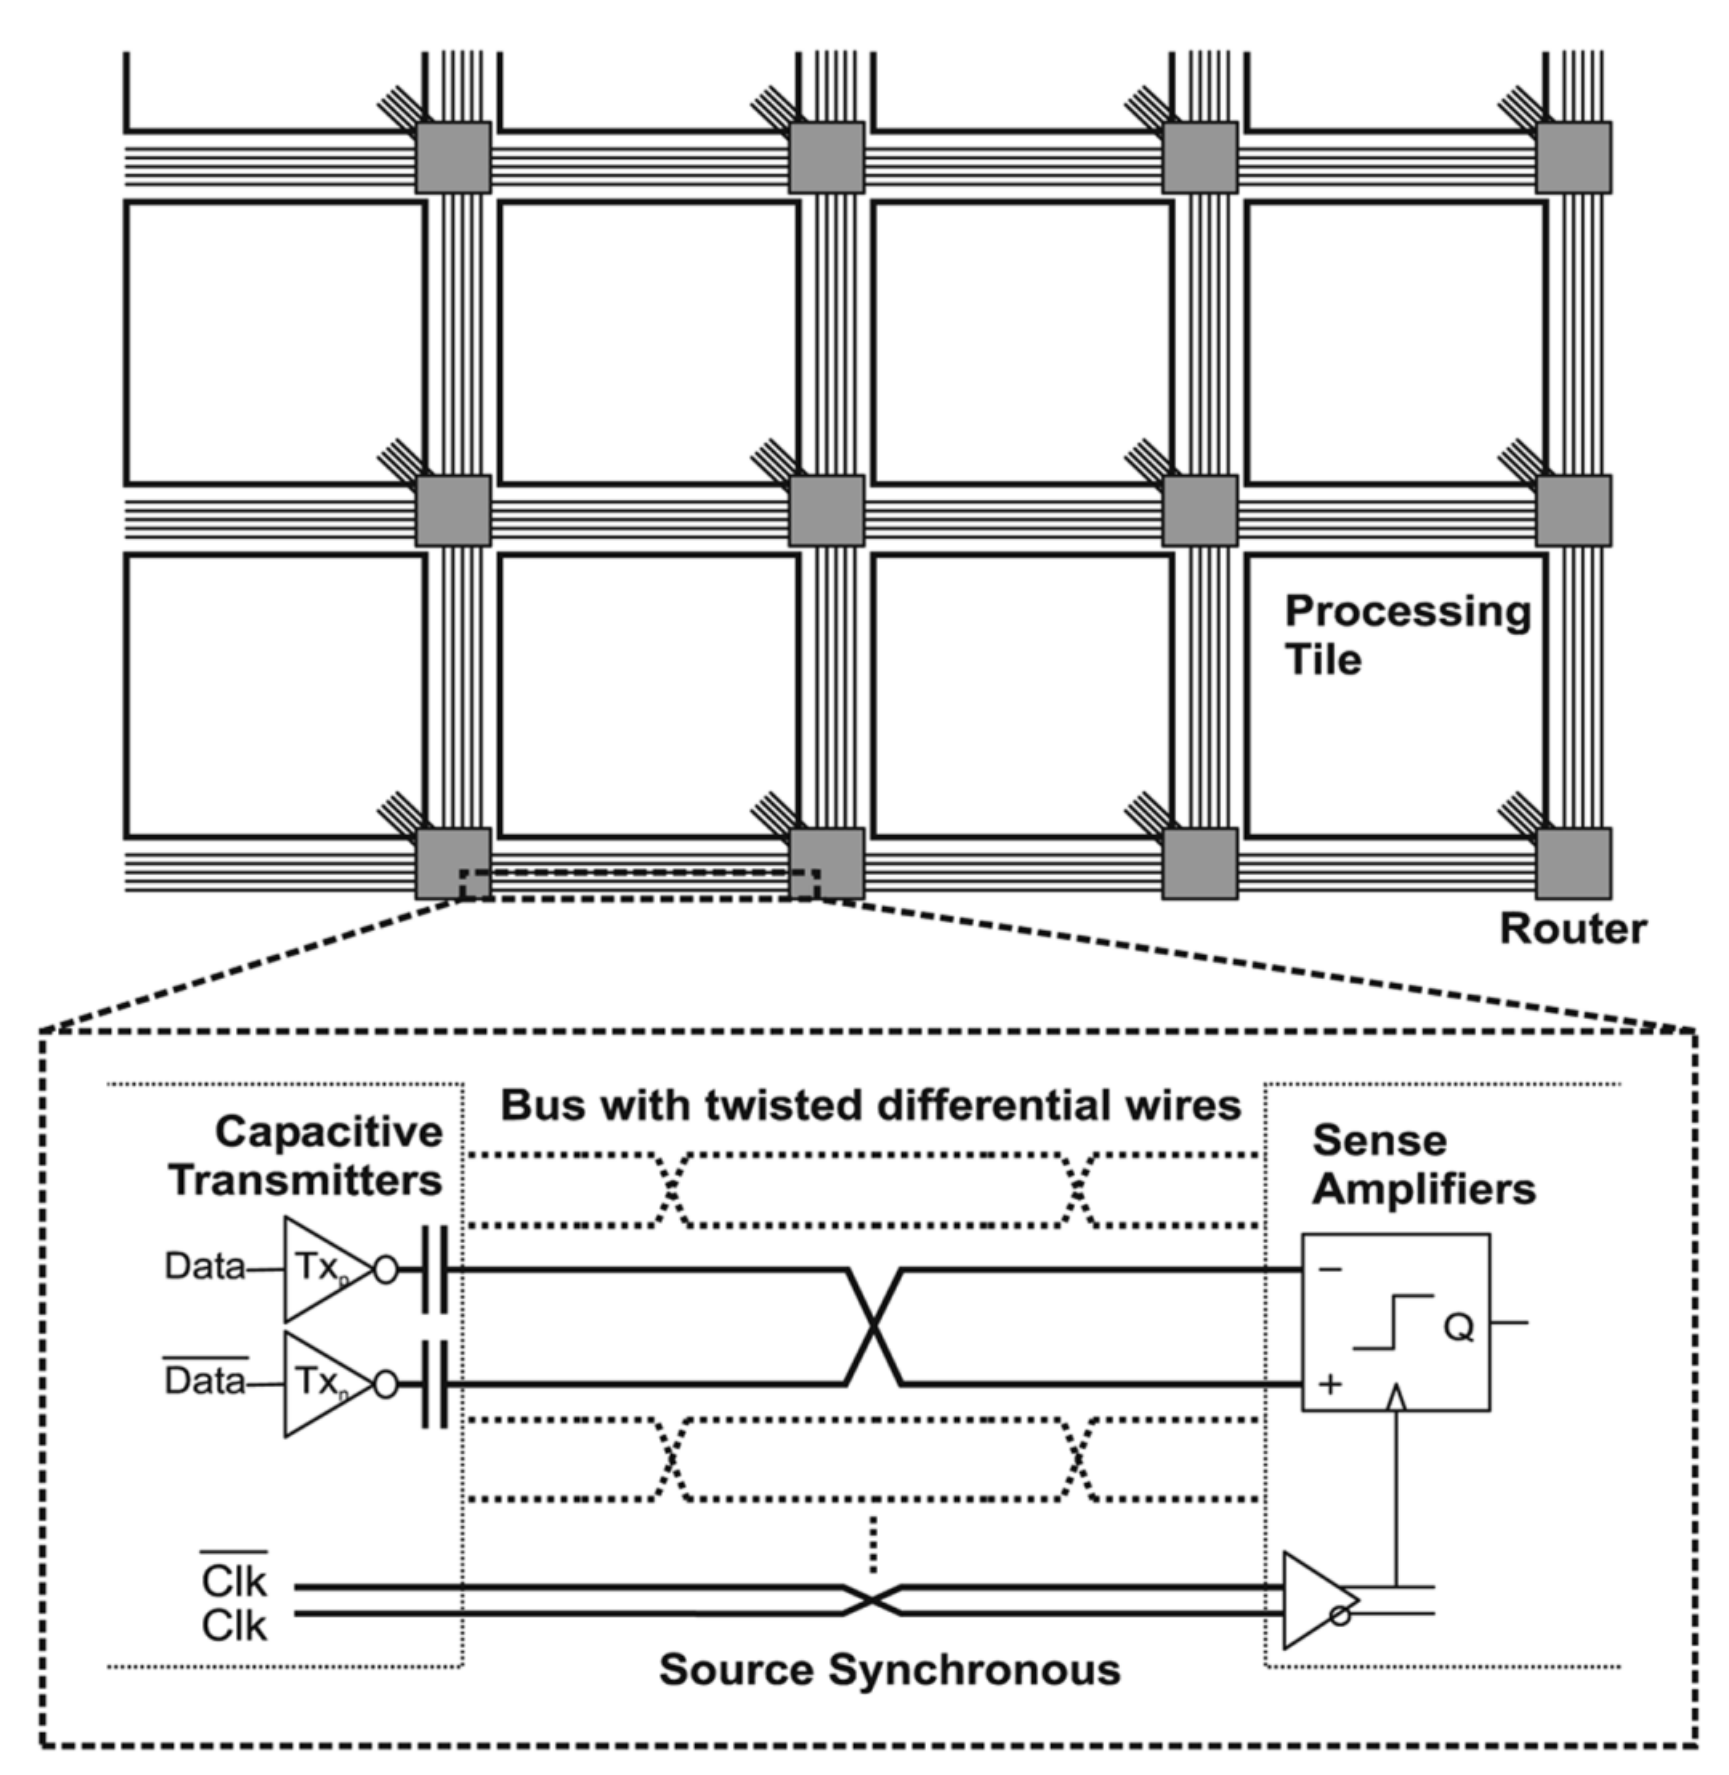
\includegraphics[width=0.78\linewidth]{Figures/Rep2Overview.png}
	\caption{Overview of the proposed transceiver for \acsp{noc}, Source: \cite{schinkel2009low}.} 
    \label{fig:rep2:overview}
\end{figure}

It is also assumed that the interconnects are unidirectional were bidirectional designs complication the design of fast transceivers.

The authors have implemented a set of optimization's which gave the improved performance:
\begin{itemize}
    \item The transmitters uses a series capacitance
    \item The interconnect consists of twisted pairs
    \item An improved sense amplifier
\end{itemize}

\subsection{Interconnect} \label{sss:rep2:interconnect}
Conventional transceivers are not suitable because its delay can vary due to crosstalk.
Crosstalk decreases the noise margin.
A Standard technique to limit crosstalk is the use of shield-wires and shield-planes and to increase the spacing between wires.
For the highest possible data-rate the designer would place a shield-wire next to each signal wire.

Conventional transceivers would also need to (dis)charge large wire and driver capacitances.
A good way to reduce the power consumption is to use low-swing signaling (lower Vdd) but this reduces the noise margin.

Use of \textit{twisted differential wire} can reduce crosstalk and allow for lower power consumption. 
The increase in area and power is relatively small, because shield-wires are not necessary anymore.
However, a sensitive differential sense amplifier is needed with a high power-supply rejection and that can reliably operate at low noise margins (see: \cref{sss:rep2:senseamp}).

The use of twisted differential wires can mitigate crosstalk only needing one twist in an even pair and two twists in an odd pair \cite{mensink2007optimal}.


\subsection{Transmitter}
% As can be seen in \cref{fig:rep2:overview}
Because the link power has a significant part in the total power usage, it is desirable to reduce the link power. 
This is for instance achieved by implemented active circuits that allow for switching between High signal swing ($V_{DDH}$) and Low signal swing ($V_{DDL}$) called a Multi-$V_{DD}$ low-swing. 
However, these circuits come with their drawback. 
For instance, the noise-margin is directly related to the power supply noise. 
A short dip in one of the two supplies could introduce a bit-error.
Also, large transistors are needed to drive the interconnects with sufficient speed.

The authors propose a capacitive pre-emphasis transmitter. 
A series capacitance $C_{TX}$ is used to drive the interconnect (see: \cref{fig:rep2:overview}). 
This capacitor acts as a capacitive divider which reduces a capacitive related swing by $C_{TX} / ( C_{WIRE} + C_{TX})$ and increases the bandwidth as $C_{TX}$ gives each transition an overshoot see: \cref{fig:rep2:capovershoot}.
Also, $C_{TX}$ attenuates the supply noise in comparison to low-swing transmitters.

\begin{figure}	\centering
	
	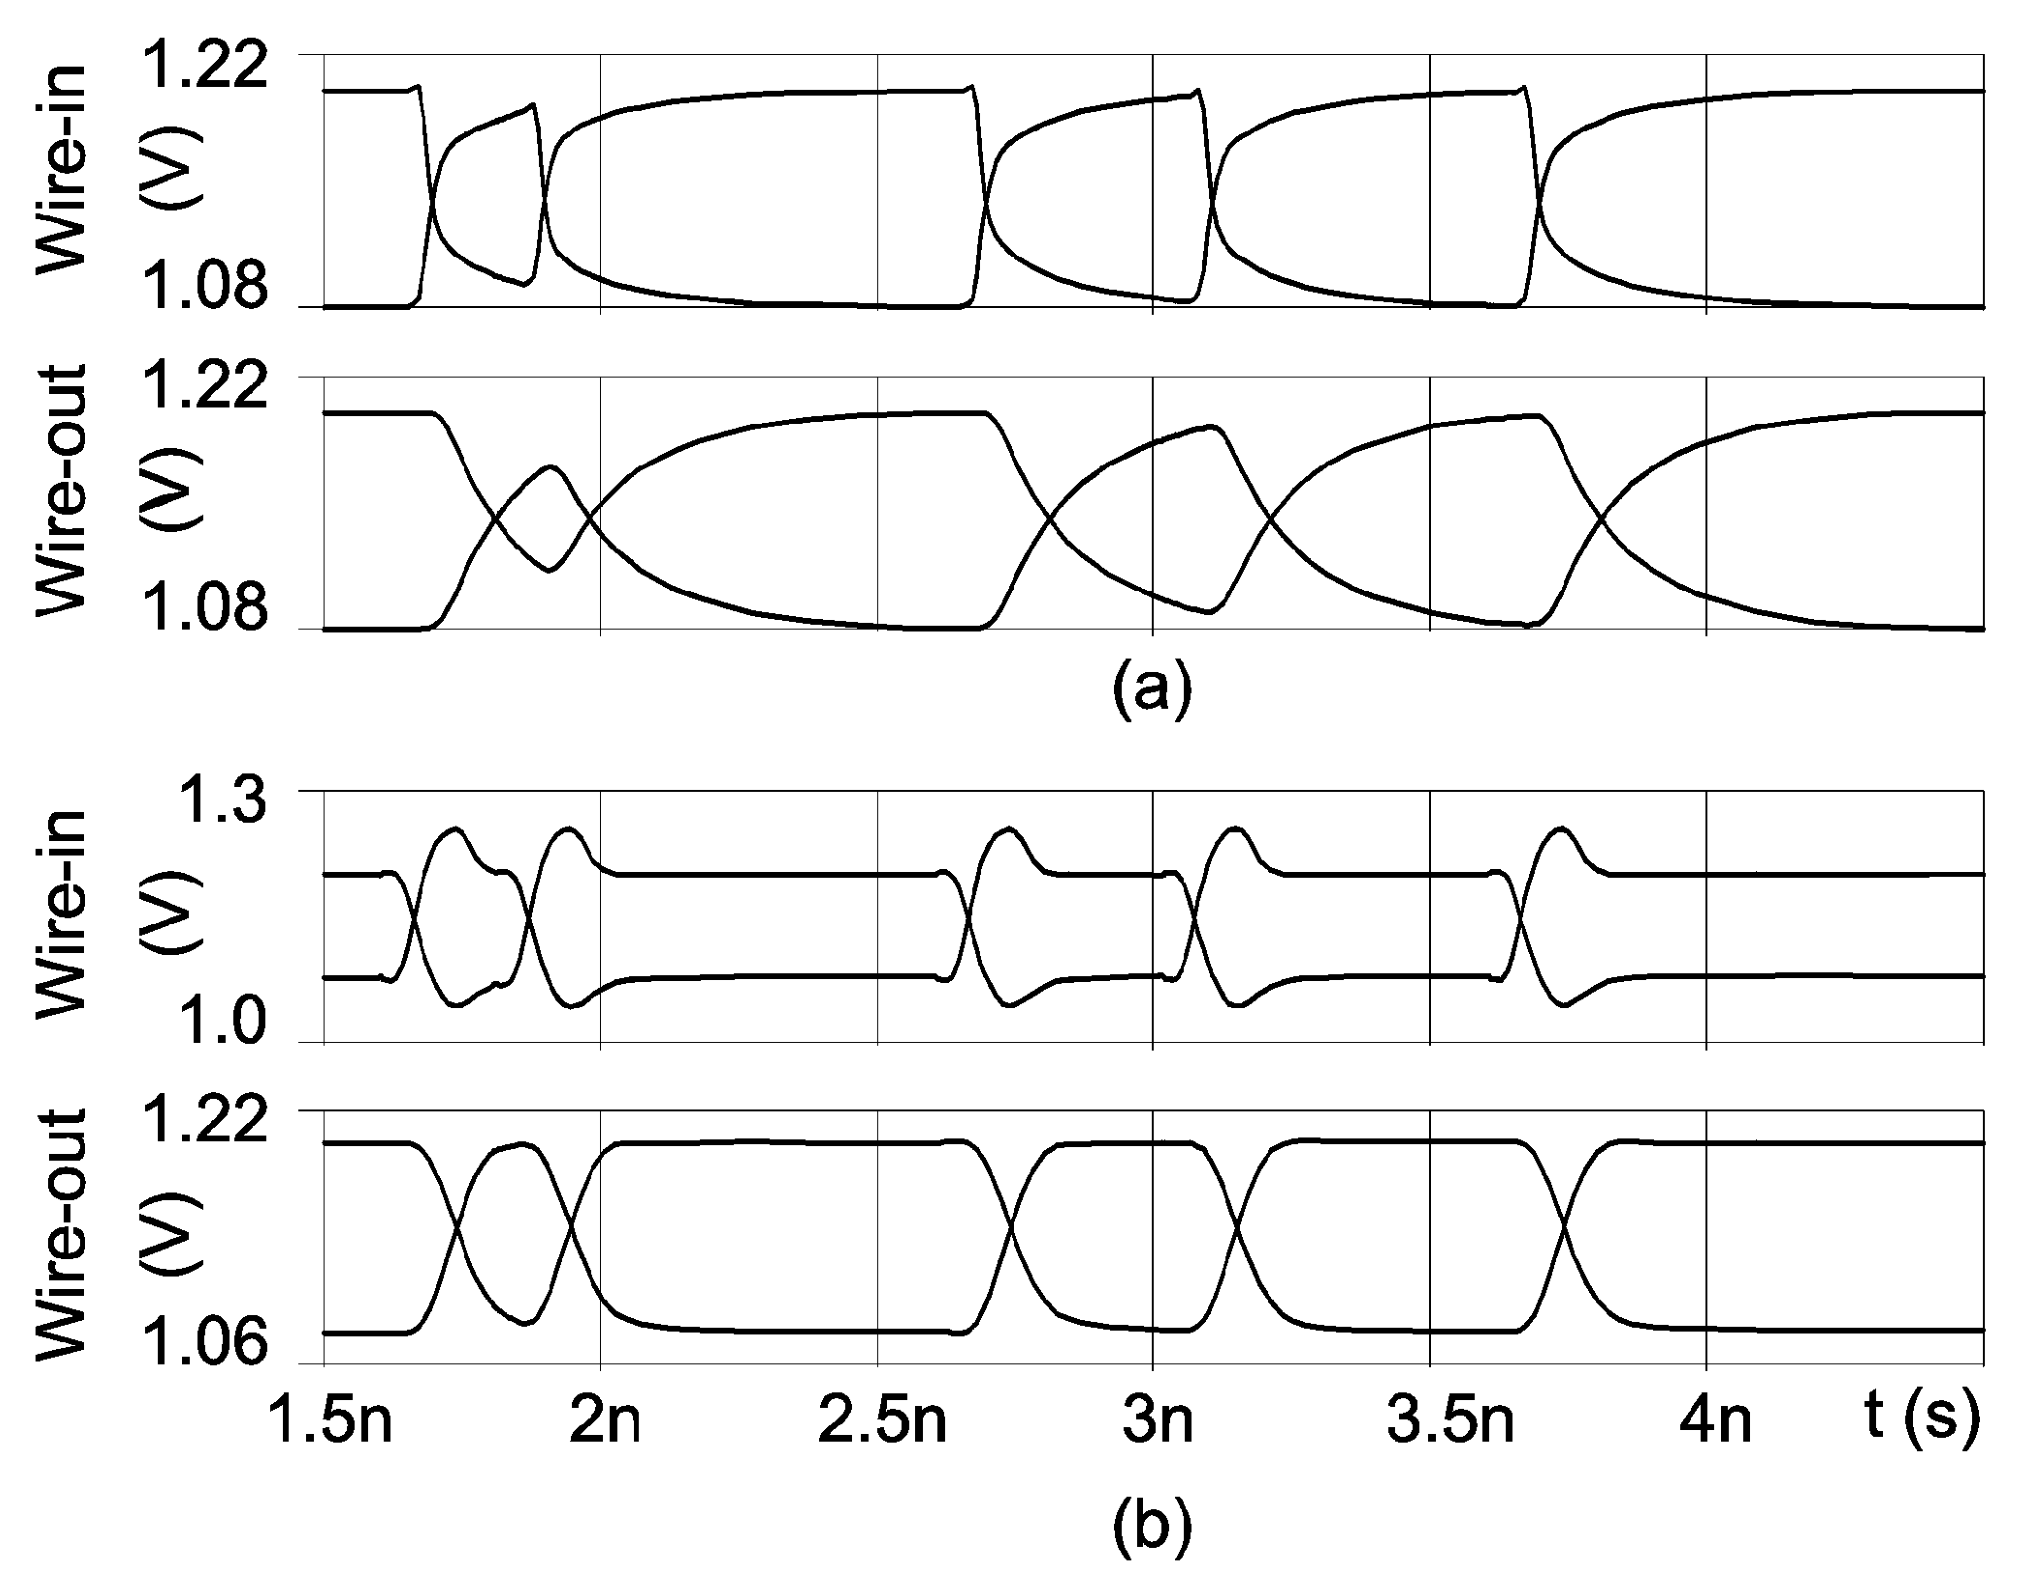
\includegraphics[width=0.8\linewidth]{Figures/Rep2TransmitterCap.png}
	\caption{Behaviour comparison of conventional transmitter (a) and a capactive transmitter (b), Source: \cite{schinkel2009low}.} 
    \label{fig:rep2:capovershoot}
\end{figure}

The capacitive transmitter has a 25 fJ overhead were a Multi-$V_{DD}$ low-swing setup uses 127 fJ per swing.



\subsection{Sense amplifier} \label{sss:rep2:senseamp} %IV Receiver and optimal swing

\begin{figure}
    \centering
	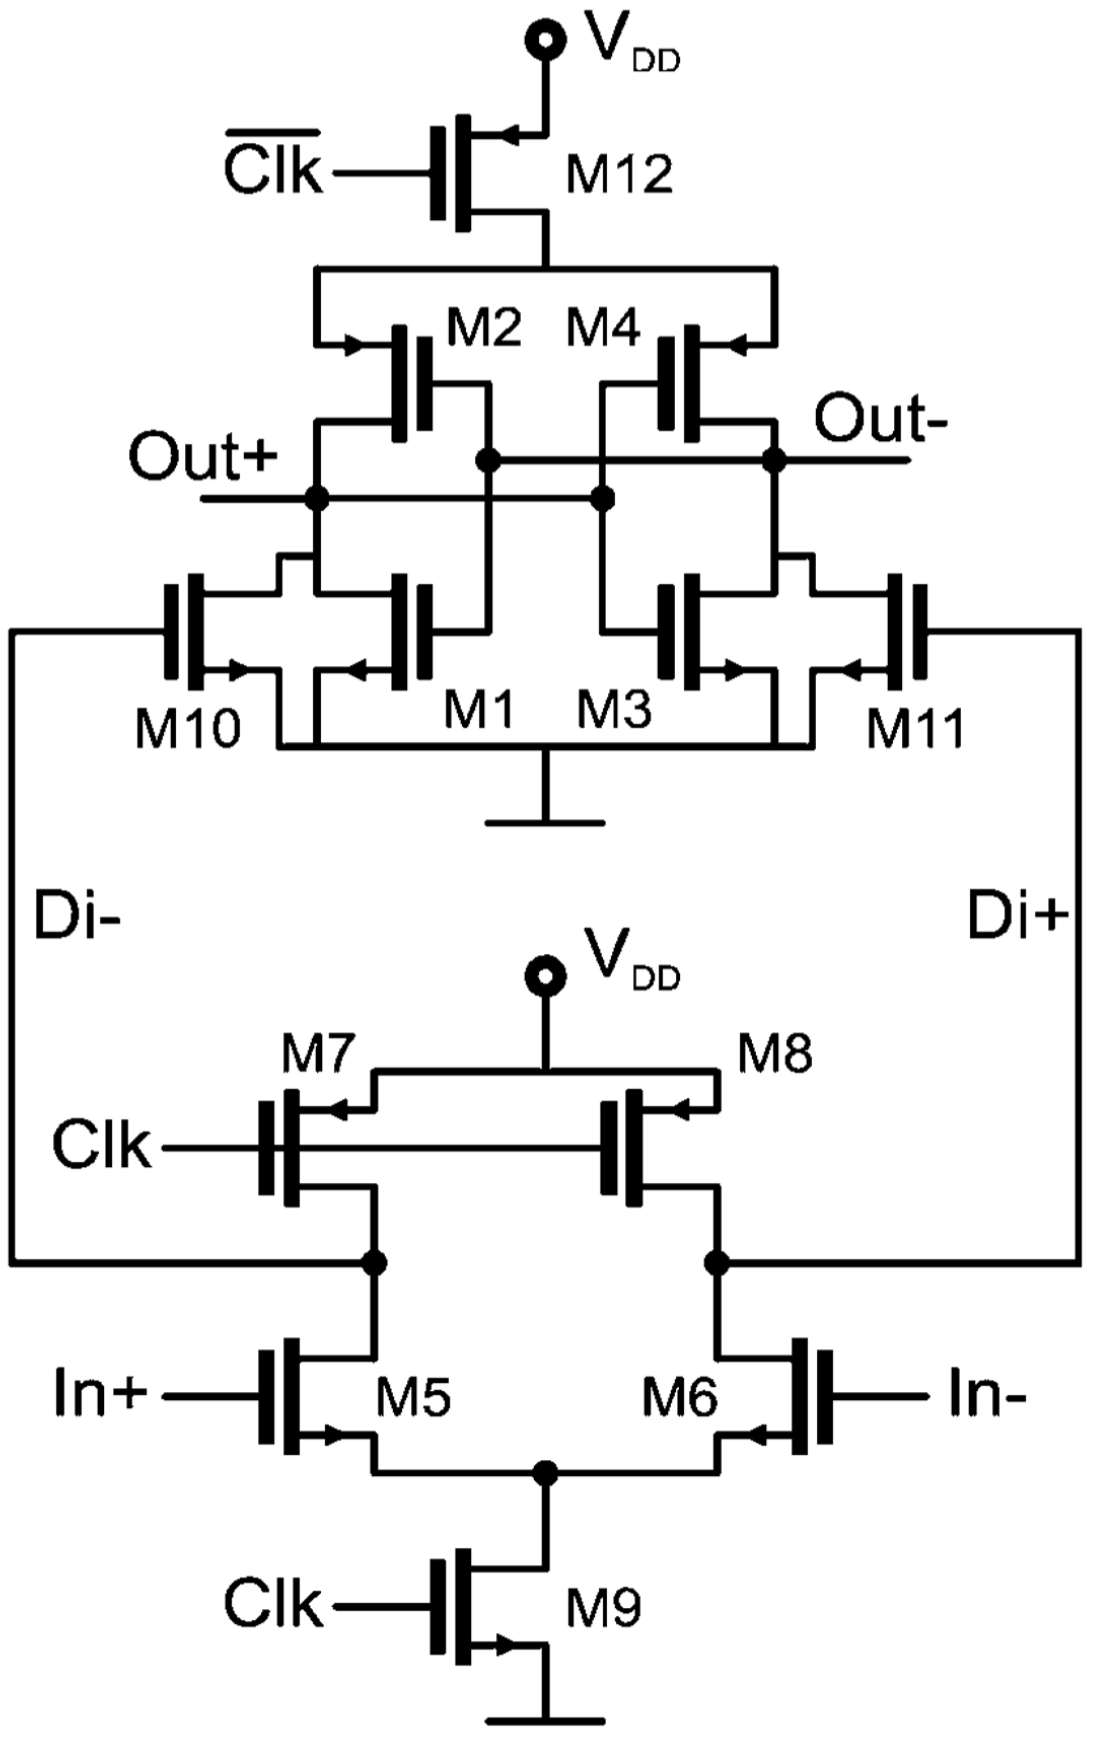
\includegraphics[width=0.6\linewidth]{Figures/Rep2DoubleTail.png}
	\caption{Double tail sense amplifier, Source: \cite{schinkel2009low}.} 
    \label{fig:rep2:doubletail}
\end{figure}

A sense amplifier not only samples incoming data fast, it also realigns it to a clock and regenerates the voltage.
The improved sense amplifier is based on the \textit{double-tail} amplifier (see: \cref{fig:rep2:doubletail}, \cite{schinkel2007double}).
The upper-tail shows the latching stage and the lower-tail shows the input stage.
There is no need for dedicated reset transistors.
This topology has an extra degree of freedom because it enables optimization between speed, offset, power and common-mode voltage.

The offset is the bottleneck for the amplifier.
The transistor dimensions are optimized to get the lowest offset standard deviation per unit of power cost.

The influence of the change in technology (Dennard scaling) on the optimum swing is not present.
The $C_{wire}/length$ does not change significantly over different technologies

% The sense amplifier is able to quickly recover the the voltage to full swing and also samples incoming data .
% the improved sense amplifier which can also operate over a wide common-mode and supply voltage range.


\subsection{Transceiver} \label{sss:rep2:transceiver}
The \ac{synclink} scheme is most likely to be used in combination with the transmitter (see: \cref{fig:rep2:transceiver}).
Parallel to the capacitive transmitter a half-rate clock is transmitted ("double-data rate").
The sense amplifier consist of two parts (as described earlier).


\begin{figure}	\centering
	
	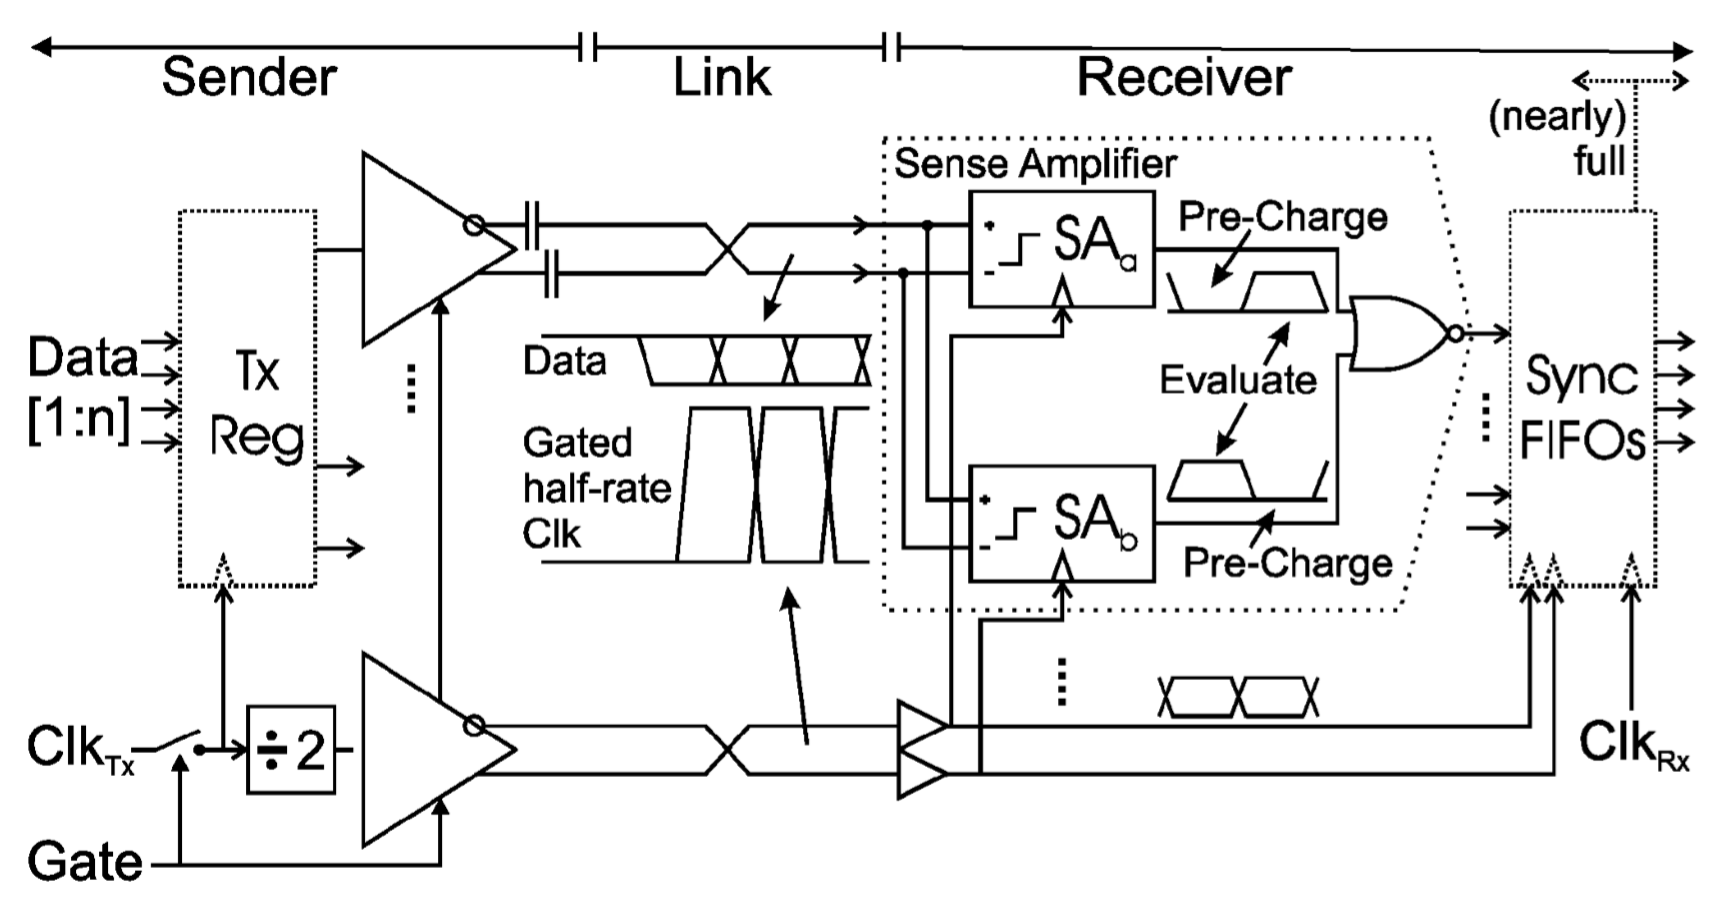
\includegraphics[width=0.9\linewidth]{Figures/Rep2Transceiver.png}
	\caption{The complete transceiver, Source: \cite{schinkel2009low}.} 
    \label{fig:rep2:transceiver}
\end{figure}

%Cascaded Transceivers

In certain routing schemes, intermediate routers can be ommitted by using direct forwarding (wave-pipeling).
To test this concept a number of cascaded transceivers were simulated.
The startup of the clock appears to be a speed-limiting factor.
Clock-wires in a two times larger metal layer (four times lower resistance) show that the system is capable to run at $9 Gb/s$.
Without this optimization it is still possible to reach $5 Gb/s$.
To test the effect of crosstalk a simulation with a bus was doen.
Almost no crosstalk was visible in the output of three neighbouring channels.

%Conclusion
The combination of a low-swing capacitive pre-emphasis transmitter, a twisted differential wires bus, a double-tail sense amplifier and a \ac{synclink} clocking is very suitable for communication in a NoC.
The circuits are compatible with standard CMOS circuits and scalable for future technologies.